\section{Temporal instability and economic usability}

This section provides supporting evidence for the real-time-use stage of the framework. Because it studies independent stock-return predictors rather than the 30 pricing-dimension networks, it does not by itself show that the latent pricing dimension changes through time. Direct evidence on the dimension comes from the Core-86 development and locked pricing tests in Section~4. The forecast replay uses future-validation eligibility and complete-state-history screens, historical preprocessing, and previously selected neural hyperparameters. It is consequently a retrospective selected-sample comparison, not a fully prospective investable backtest; lagged policy decisions alone do not remove these sample and design qualifications.

\subsection{Does routine updating improve forecasts?}

The preceding analysis shows that the selected pricing dimension changes across its two nonoverlapping Core-86 periods. A natural response is to update the model frequently. The separate return-prediction replay evaluates updating, without testing a policy for choosing pricing dimension. Across 239 months and 1,043,511 stock-month observations, the frozen neural model has mean monthly squared loss 0.034313. The rolling 60-month model has loss 0.034451, and the expanding-history model has loss 0.034762. Relative to a zero forecast, their $R^2$ values are 0.261\%, $-0.140$\%, and $-1.042$\%. The point estimates favor the frozen model, although the inference does not establish that updating is universally harmful.

The full-sample average hides temporal heterogeneity. Equation~\eqref{eq:update-decomp} separates the magnitude of each model change from whether that change points toward subsequently realized returns. The two loss columns in Table~\ref{tab:temporal-economic} report the resulting update-minus-frozen differences for all three learners. For the neural model, the underlying components explain the change of sign. For rolling updates in 2000--2009, adjustment cost $A=0.000583$ dominates alignment benefit $2B=0.000051$, so updating raises loss by 0.000531. In 2010--2019, adjustment is smaller and alignment rises to 0.000509, producing a loss improvement of 0.000252. The ex-post optimal shrinkage intensity $\lambda^*=\operatorname{clip}(B/A,0,1)$ moves from 0.044 to 0.991. Expanding neural updates do not show the same reversal: their alignment remains too weak in both decades.

\begin{widetable}[!tbp]
\centering
\begin{minipage}{\textwidth}
\caption{Forecast updating and portfolio performance by learner and update rule}
\label{tab:temporal-economic}
\footnotesize
\setlength{\tabcolsep}{4pt}
\renewcommand{\arraystretch}{1.16}
\begin{tabular*}{\linewidth}{@{\extracolsep{\fill}}llrrrrrr@{}}
\toprule
 &  & \multicolumn{2}{c}{Updated minus frozen loss} & \multicolumn{4}{c}{Value-weighted portfolios; 25 bp cost} \\
\cmidrule(lr){3-4}\cmidrule(l){5-8}
Learner & Rule & 2000--09 & 2010--19 & Return (\%) & Sharpe & Turnover & CE (\%) \\
\midrule
Neural & Frozen & 0.000 & 0.000 & 13.02 & 0.546 & 1.219 & -1.20 \\
 & Rolling 60 & 0.531 & -0.252 & -0.61 & -0.022 & 0.874 & -20.32 \\
 & Expanding & 0.806 & 0.094 & 13.12 & 0.444 & 1.352 & -8.68 \\
\addlinespace[5pt]
Ridge & Frozen & 0.000 & 0.000 & 5.59 & 0.245 & 0.787 & -7.47 \\
 & Rolling 60 & 2.040 & 0.013 & 4.60 & 0.158 & 1.030 & -16.63 \\
 & Expanding & 0.031 & -0.331 & 7.92 & 0.378 & 0.745 & -3.04 \\
\addlinespace[5pt]
Tree & Frozen & 0.000 & 0.000 & 3.83 & 0.120 & 1.030 & -21.55 \\
 & Rolling 60 & 1.122 & -0.873 & -11.65 & -0.371 & 1.324 & -36.23 \\
 & Expanding & -0.771 & -1.650 & -0.16 & -0.005 & 1.148 & -22.38 \\
\bottomrule
\end{tabular*}
\par\vspace{4pt}
{\footnotesize\raggedright\textit{Notes:} Loss differences are multiplied by $10^3$; negative values favor updating. Zero for the frozen rule is the comparison baseline. Portfolio return and certainty equivalent (CE, risk aversion five) are annualized percentages over February 2000--December 2019. Turnover is monthly for unit long and unit short positions after return drift. Portfolio columns cover the full period, not the individual decades in the loss columns. These are separate return-prediction learners, not the pricing-dimension networks. None of the six update-minus-frozen return differences passes the Holm-adjusted 5\% gate.\par}
\end{minipage}
\end{widetable}


The identity has an economic interpretation. A model can adapt strongly and still fail because its changes are orthogonal to, or negatively aligned with, subsequent errors. Conversely, a modest change can add value if it consistently corrects the frozen error. ``Parameter drift'' is therefore insufficient. The direction of the drift relative to future pricing mistakes is what matters.

\subsection{Cross-estimator evidence and memory length}

Ridge and shallow tree models help separate a neural-network peculiarity from a broader updating tradeoff. For rolling 60-month estimates, both the neural and tree models move from adjustment-cost dominance in the 2000s to alignment-benefit dominance in the 2010s. The tree update changes from a loss increase of 0.001122 to a loss reduction of 0.000873. Ridge rolling updates improve substantially but remain slightly costly in the second decade.

Long-memory results are estimator-specific. Expanding Ridge improves the frozen forecast in the 2010s, and the expanding tree improves it in both decades; expanding neural updates do not. No update window is universally optimal. What travels across model classes is a higher alignment of model changes with subsequent frozen-model errors in the later sample, especially for short-memory fits. The economic tradeoff is between responsiveness to drift and estimation variance, and that tradeoff depends on the learner.

High realized stock-market variance raises losses for all three neural policies. The high-variance state is the only one of four frozen environment definitions that remains significant for all policies after Holm adjustment and across HAC bandwidths. This result does not prove a change in the conditional-mean mapping, because the squared-error target mechanically contains more return noise in volatile months. It is reported as performance heterogeneity, not structural attribution.

\subsection{Retrospective change versus real-time detection}

Using the full 2000--2019 sample, the six standardized model--window advantage series share an estimated break after April 2014. The exploratory joint block-bootstrap $p$-value is 0.0214, and all six mean changes are positive. The bootstrap interval for the first post-break month runs from October 2009 to January 2015, however, which is wide relative to a real-time trading horizon.

The historical CUSUM exercise is more demanding. Its threshold of 5.6178 is calibrated on 2000--2009 to target a nominal 5\% probability of one or more false triggers over 120 months under the bootstrap calibration distribution. The statistic does not cross that threshold until August 2018; updating begins in September and is active for only 16 of the 120 evaluation months. The neural switch improves on the frozen model by only 0.000048 per month, with a confidence interval containing zero and Holm $p=1.000$. It underperforms always rolling by 0.000204, with Holm $p=0.0405$. Ridge and tree switch rules also fail their prespecified advancement comparisons.

This gap between 2014 and 2018 is central. A change can be detectable after accumulating the complete post-break record and still be too weak or gradual to identify promptly under false-alarm control. Lowering the threshold after observing the delay would use future information and turn a failed test into specification search. The frozen rule is therefore closed rather than tuned.

\subsection{Portfolio implementation}

The portfolio columns in Table~\ref{tab:temporal-economic} evaluate the same learner--rule combinations over the full period under the primary value-weighted, 25-basis-point specification. These columns test economic usefulness separately from the decade-specific forecast losses. The frozen neural strategy has the largest Sharpe ratio, 0.546, and annualized net return of 13.02\%. Rolling neural updating reduces the return to $-0.61$\% and raises no economic-use claim. Expanding neural updating has a similar return to the frozen policy but a lower Sharpe ratio. Ridge expanding performs better than frozen Ridge in point estimates, while both tree updates are weaker than frozen tree.

None of the six update-minus-frozen return differences survives the prespecified Holm 5\% gate. The neural rolling policy trails frozen by 1.136 percentage points per month; its unadjusted $p=0.0122$ becomes Holm $p=0.0732$. The positive Ridge-expanding difference has an interval containing zero and Holm $p=1$. Every value-weighted strategy has a negative certainty equivalent at risk aversion five.

Costs materially affect ranking. The frozen neural annualized return falls from 16.68\% with zero cost to 9.36\% at 50 basis points. Ridge expanding falls from 10.15\% to 5.68\%, and tree expanding from 3.29\% to $-3.60$\%. The result is consistent with the broader point that model comparison can change after turnover is priced \citep{detzel2023costs}. Predictive updating and economic updating are distinct endpoints.

Figure~\ref{fig:temporal-dashboard} links the three temporal hurdles: forecast adjustment can reverse sign across decades, the real-time rule detects the retrospective break with a long delay, and every primary after-cost certainty equivalent remains negative.

\begin{widefigure}[!tbp]
\centering
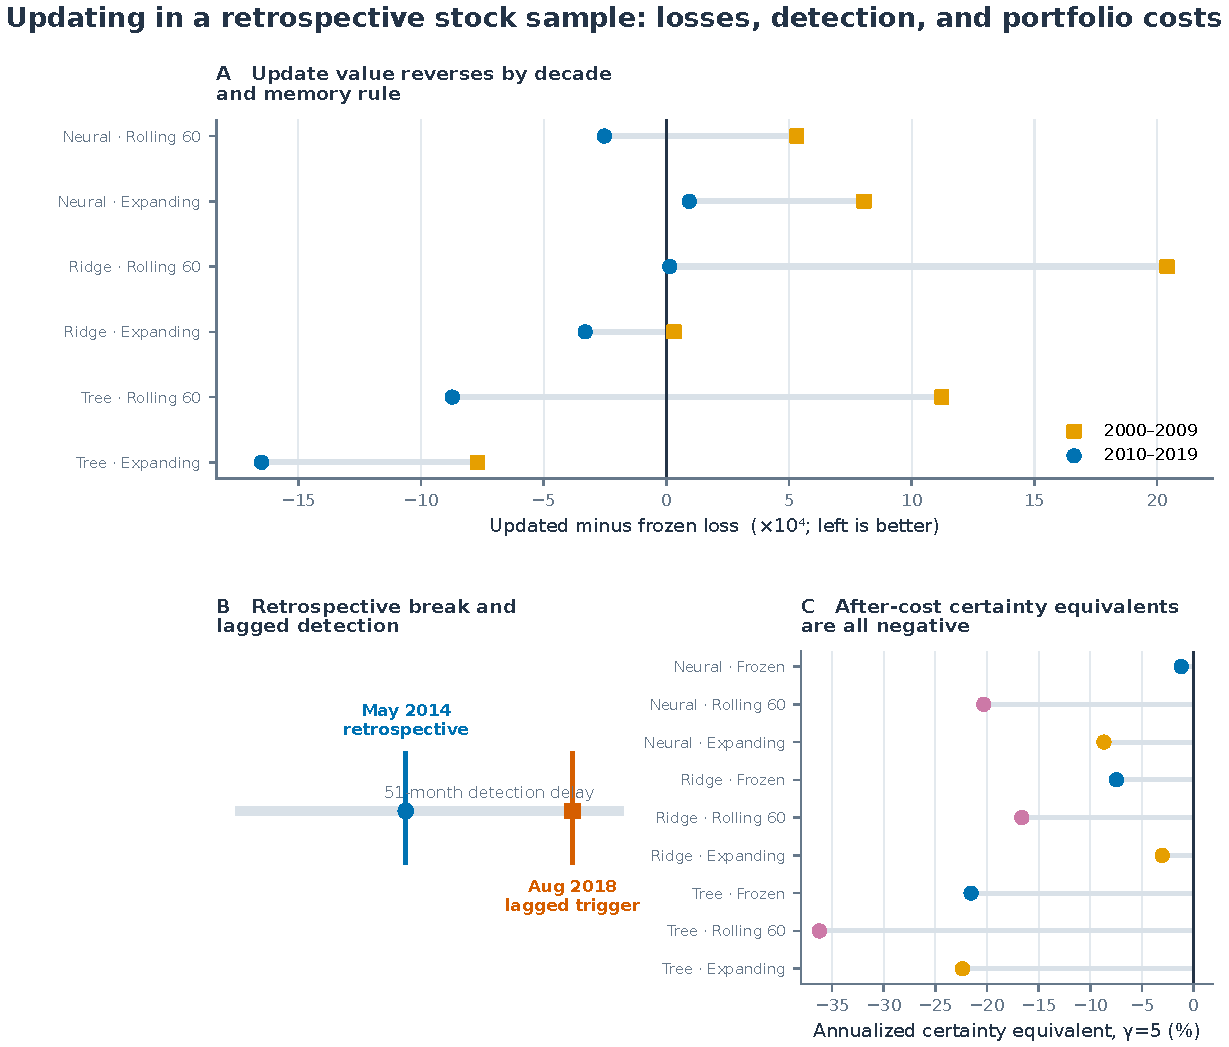
\includegraphics[width=0.99\textwidth]{figures/figure_06_temporal_usability.pdf}
\caption{Temporal usability dashboard. Panel A reports updated-minus-frozen loss by learner, memory rule, and decade. Panel B contrasts the exploratory retrospective break with the frozen real-time CUSUM crossing. Panel C reports annualized certainty equivalents for the value-weighted 25-basis-point primary portfolios.}
\label{fig:temporal-dashboard}
\end{widefigure}

\subsection{Implication for temporal dimension claims}

Temporal instability does not imply that a researcher should continually change $K$ or retrain every parameter. A low-dimensional representation can remain geometrically compact while the risk prices attached to its directions, its asset exposures, or the usefulness of its forecast changes evolve. The current evidence locates a change in update alignment, but it does not yet separate exposure-span rotation from risk-price migration in the full 30-model family. That attribution is outside the evidence reported here.

For the evidence available here, the appropriate conclusion is narrower. Updating value varies over time and can be visible retrospectively. The tested lagged detector does not identify that change early enough to establish incremental value in this internal replay. Therefore a time-varying pattern cannot be used as evidence for a stable, real-time economic state variable unless the detection and implementation gates pass separately.
